\section{genericSink.h File Reference}
\label{genericSink_8h}\index{genericSink.h@{genericSink.h}}
{\tt \#include \char`\"{}../interfaces/processor.h\char`\"{}}\par
{\tt \#include \char`\"{}../../data\_\-types/impl/highLevelPacket.h\char`\"{}}\par
{\tt \#include \char`\"{}genericEvents.h\char`\"{}}\par
{\tt \#include \char`\"{}genericData.h\char`\"{}}\par
{\tt \#include \char`\"{}genericInterface.h\char`\"{}}\par
{\tt \#include \char`\"{}../../tests/MersenneTwister.h\char`\"{}}\par
{\tt \#include $<$deque$>$}\par
{\tt \#include $<$fstream$>$}\par


Include dependency graph for genericSink.h:\nopagebreak
\begin{figure}[H]
\begin{center}
\leavevmode
\includegraphics[width=420pt]{genericSink_8h__incl}
\end{center}
\end{figure}


This graph shows which files directly or indirectly include this file:\nopagebreak
\begin{figure}[H]
\begin{center}
\leavevmode
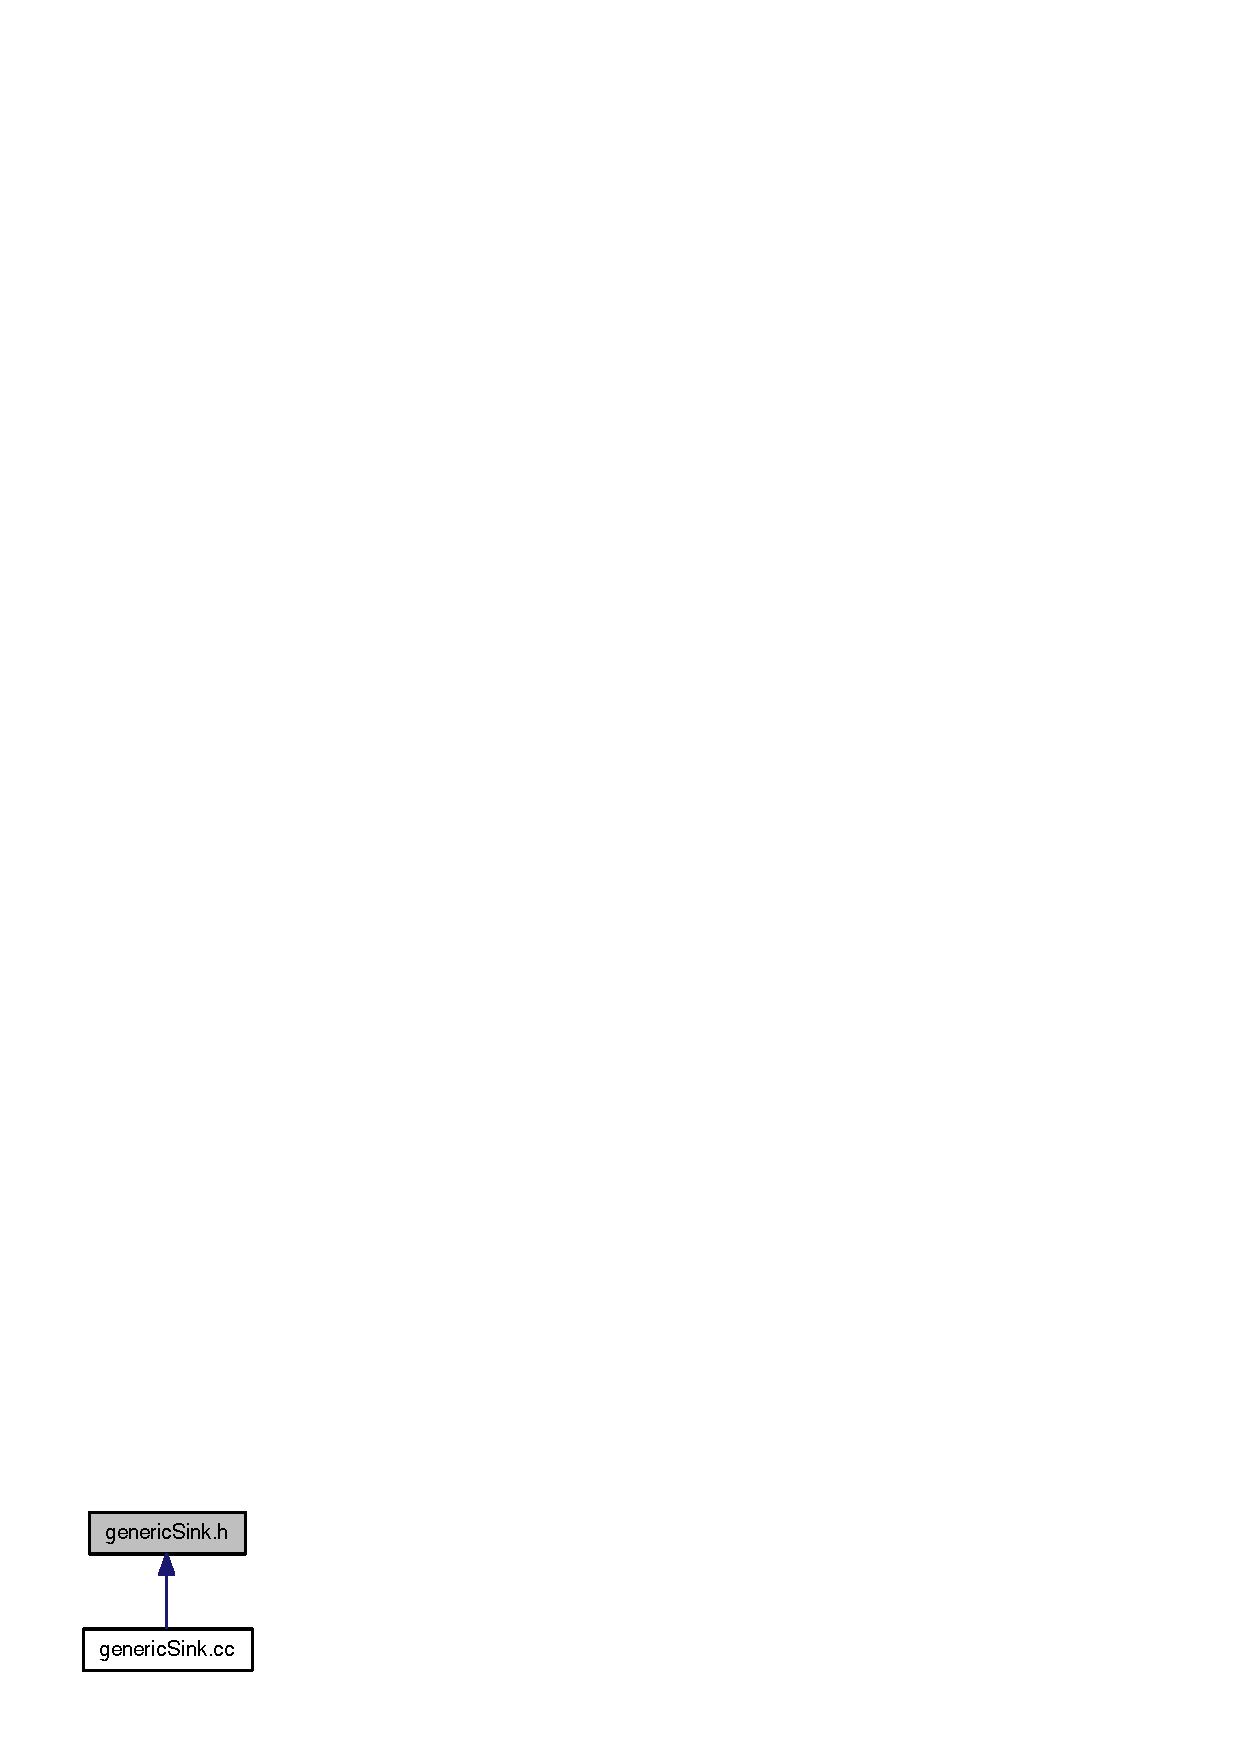
\includegraphics[width=62pt]{genericSink_8h__dep__incl}
\end{center}
\end{figure}
\subsection*{Classes}
\begin{CompactItemize}
\item 
class {\bf GenericSink}
\end{CompactItemize}
